\chapter{システム実験の詳細}
\label{chap:system}
システム実験では全3回にわたる実験を行い,被験者同士の対戦を行う第3回以外の2回は被験者がAIとの対戦とAIを用いた振り返りを行う.
第4章と同様に3回セットの実験のうち,1回目と2回目を第1段階・3回目を第2段階と呼ぶ.
以下で被験者のデータの詳細を述べ,それから実験設定や結果の詳細を段階ごとに述べていく.
\section{被験者のデータ}
実験対象者は計22人の10代-20代学生(男性17名:女性5名)であり,表\ref{table:before}に示す各種の事前質問($1\sim5$の値で答える)の結果は以下となった.
ボードゲームの経験を問う質問に関しては1を「1年に1回程プレイする」程度,5を「週に2,3回以上プレイする」程度と定めた.
connect4の経験を問う質問に関しては1を「connect4を知らない」程度,5を「週に2,3回以上プレイする」程度と定めた.
また,機械学習・強化学習の知識を問う質問に関しては1を「言葉を聞いたことがある」程度,5を「機械学習についての入門書を読んだり,授業を受けたことがある」程度と定めた.
また,被験者には先述のAllis\cite{allis}による9strategyをはじめとしたconnect4の知識的解法をネット検索等の手段で調べないよう要請した.
\begin{table}[H]
    \caption{事前質問項目:システム実験}
    \label{table:before}
	\small
    \begin{tabular}{c||c}
        \multicolumn{1}{c}{質問} & 回答の平均\\ \hline \hline
        ボードゲームの経験はどれくらいありますか & 2.18\\
        connect4(ゲーム)の経験はどれくらいありますか& 1.64\\\hline
        機械学習に対する知識はどれくらいありますか& 3.59\\
        強化学習に対する知識はどれくらいありますか& 3.23\\
    \end{tabular}
    
\end{table}
\section{第1段階}
第1段階はAIとの対戦とその振り返りによって構成されている.
振り返りモードでは表示する進行図の手数,AIの強さを被験者ごとに変更しつつ実験を行った.
進行図の手数は$\{3, 5, 7, 制限なし(最後まで表示)\}$の4段階,AIの強さは$\{強,弱\}$の2段階を設定した.
また,対戦を行うAIモデルを用いて振り返りの進行図を生成した.
使用したAIモデル(alphazero\_baseline),提案手法に与えるパラメータを表\ref{table:param-system}に示す.
\begin{table}[H]
	\caption{AIモデルのパラメータ(システム実験・第1段階)}
    \label{table:param-system}
	\centering
	\scalebox{0.98}[0.98]{
		\begin{tabular}{c|c|c}
			モデル&強&弱\\\hline
			time    & 5 & 1 \\ 
			$C_{puct}$ & 1   & 0.25 \\
            エポック数 & 200 & 1 \\
			$k$ (提案手法のみ)     & 4 & 4 \\
			$l$ (提案手法のみ)     & 2 & 2 \\

		\end{tabular}
	}
	
\end{table}
また,1回の実験当たりの制限時間は7分とし,実験内のAIとの対戦は2回までに制限した.
これは実戦経験による熟達ではなく支援システムによる学習過程の観察という実験の趣旨に従うためである.
\subsection{振り返りモード(GUI)の詳細}
振り返りモードでは直前の対戦の内容を振り返ることができる.
「>/<」ボタンを押すことで「1つ先の盤面に進む/戻る」ことができる.
また,振り返りを補助する機能として画面左下の「counts」に表示されている盤面$s$に対する
各行動の訪問回数$N(s)$,「value」に局面評価$V(s)$を示した.
$N(s),V(s)$は対戦に使用したモデルから導かれる.
数字が書かれているボタンはAIモデル(対戦に使ったモデルと同じ)による進行図を提示するボタンであり,ボタンに描かれた数字
と同じ列を選択した場合の進行図を見ることができる.
図\ref{fig:number-button}では「4」と描かれたボタンを押した結果,左から4番目を選択した場合の進行図が表示されていることがわかる.
選択した位置は「*」マークで表示される.
\begin{figure}[t]
	\centering
    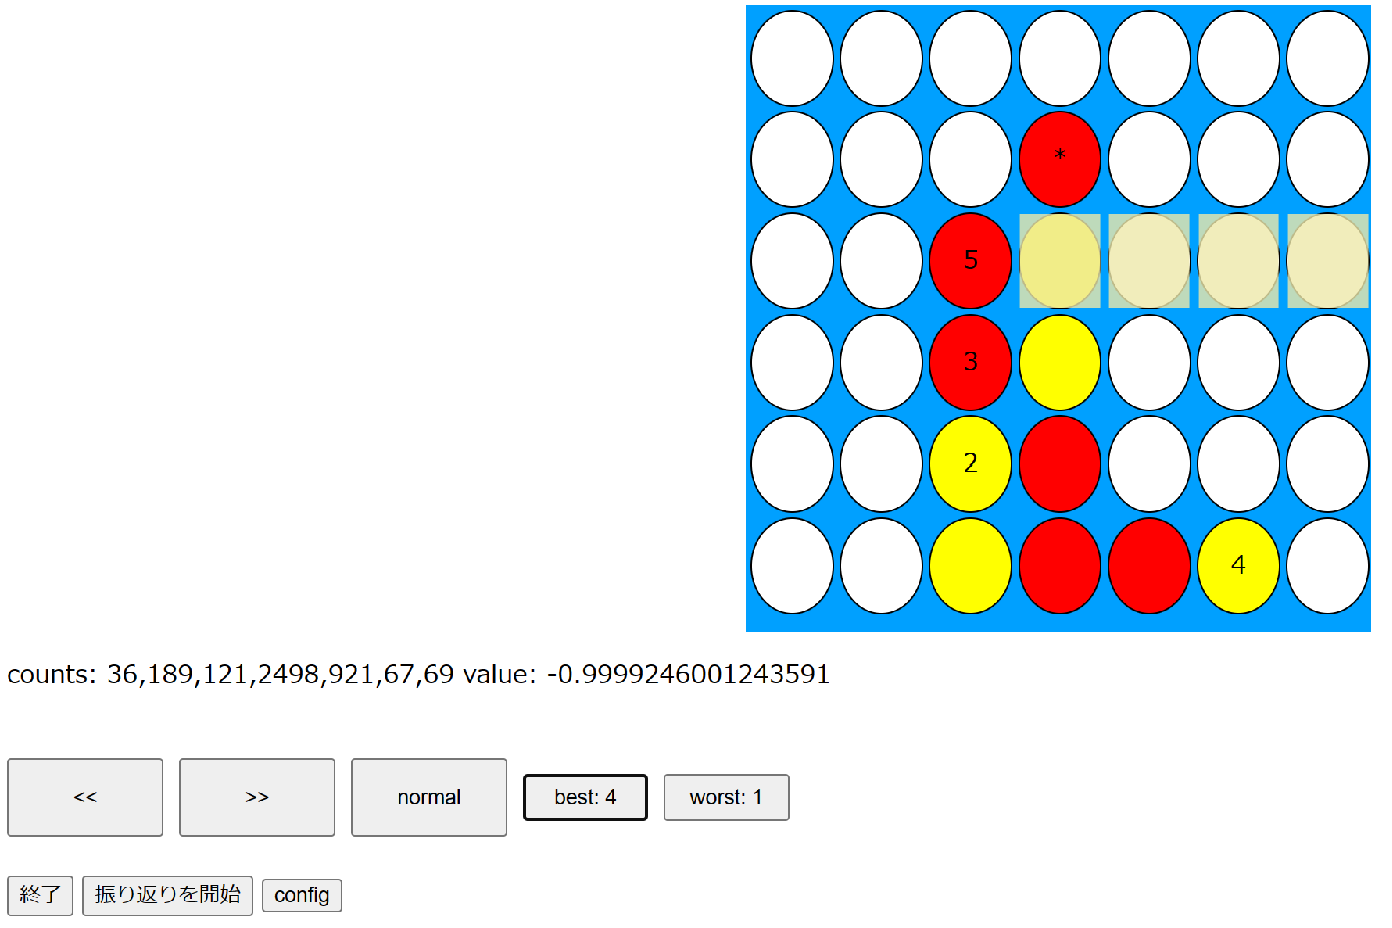
\includegraphics[width=\linewidth]{./figure/trajSystem.pdf}
	\caption{進行図の提示}
	\label{fig:number-button}
\end{figure}
想定図中の数字は数字の大きさの順番に石が置かれるというAIの予想を表している.図\ref{fig:multi}
では赤が「*」マークの位置に石を置いた次に黄は左から3列目の位置,その次に赤は左から3列目に打つことが予測されている.
また,図中で色づけられている部分は進行図においてその部分がは4つ以上つながることを示している.赤く色づけられている場合はその部分で
赤が4つ以上つながると予想されていること,黄色く色づけられている場合はその部分で黄色が4つ以上つながると予想されているこを示している.
また,提案手法による振り返りが適用されたグループでは提示される進行図が複数となる.そのため図\ref{fig:multi}に示すように他の想定図を見ることができる「next\_prej/pre\_traj」
ボタンが追加される.
\begin{figure}[t]
	\centering
	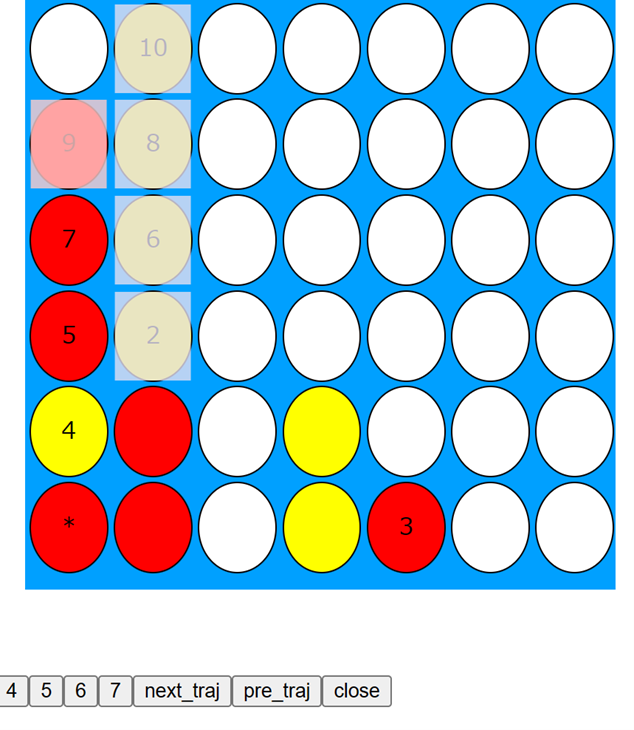
\includegraphics[width=150pt]{./figure/multi.png}
	\caption{提案手法による進行図の提示}
	\label{fig:multi}
\end{figure}
ここからは第1段階中の1日目,2日目のGUIの違いについて述べる
\subsection{1日目}
1日目は被験者の操作間への慣れを促進するため全ての選択肢に対し進行図表示ボタン(数字ボタン)を設置した.
図\ref{fig:traj-button}に示すようにこれらのボタンは「traj」ボタンを押すことで出現する.
\begin{figure}[t]
	\centering
	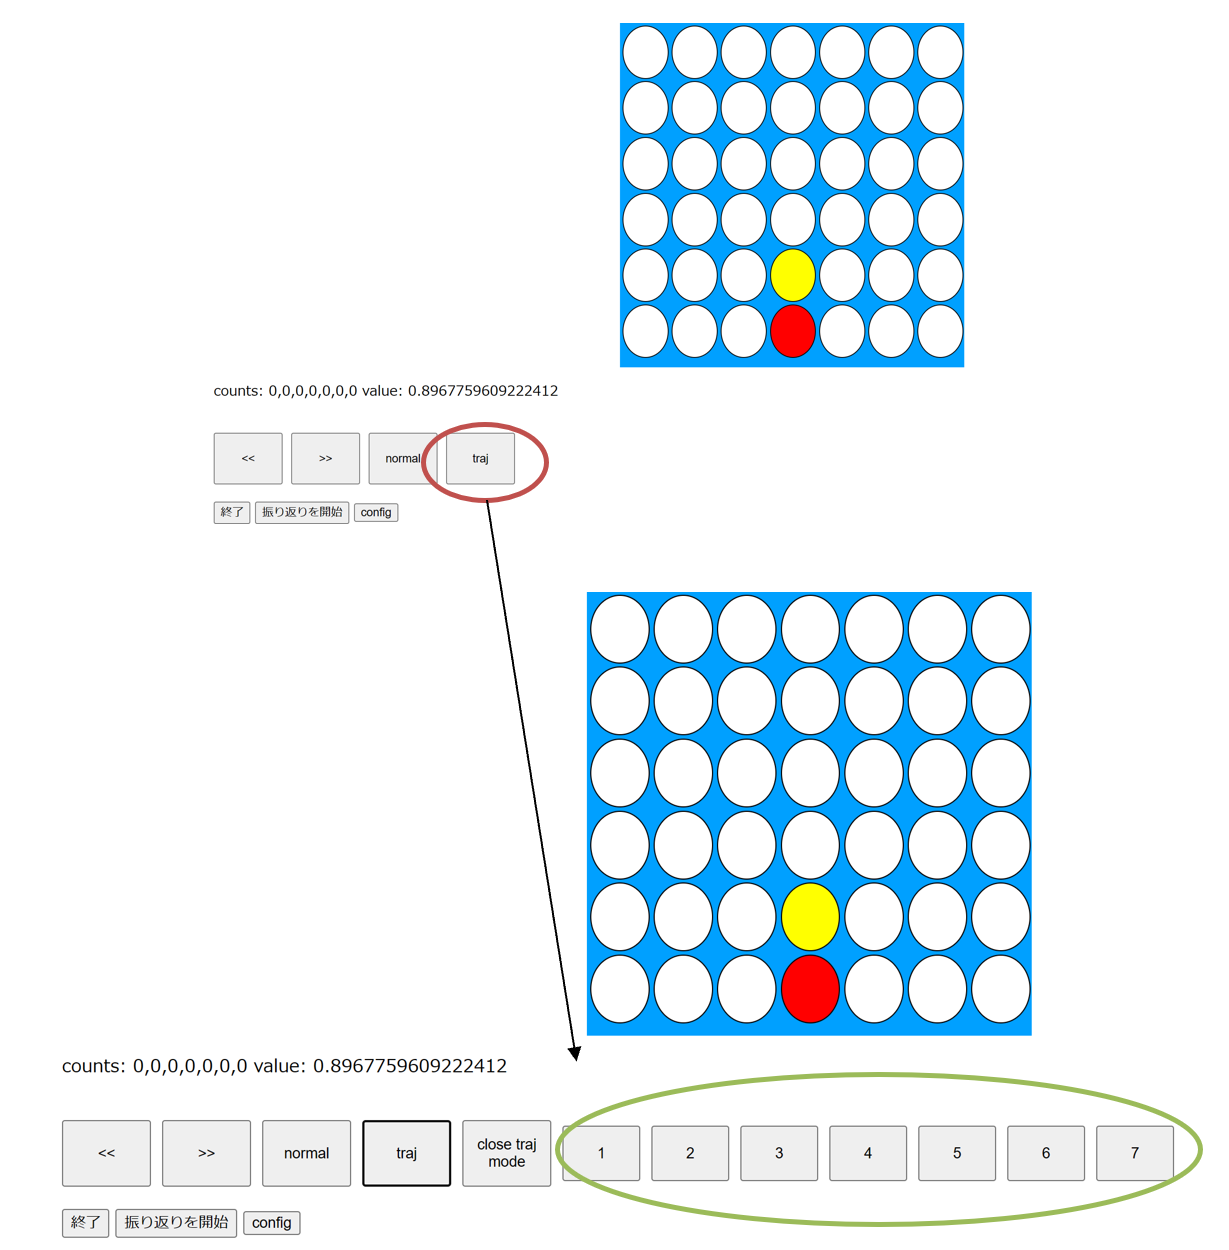
\includegraphics[width=\linewidth]{./figure/traj-button.png}
	\caption{進行図表示ボタン(1日目)}
	\label{fig:traj-button}
\end{figure}
\subsection{2日目}
2日目は進行図の閲覧を促進するためtrajボタンを廃止し,最も訪問回数$N(s,a)$の多い選択肢$a_{max}$,少ない選択肢$a_{min}$
からの進行図を示すボタンをそれぞれ「best:(列の数字)」「worst:(列の数字)」のラベルで図\ref{fig:best-worst}のように表示した.
\begin{figure}[t]
	\centering
	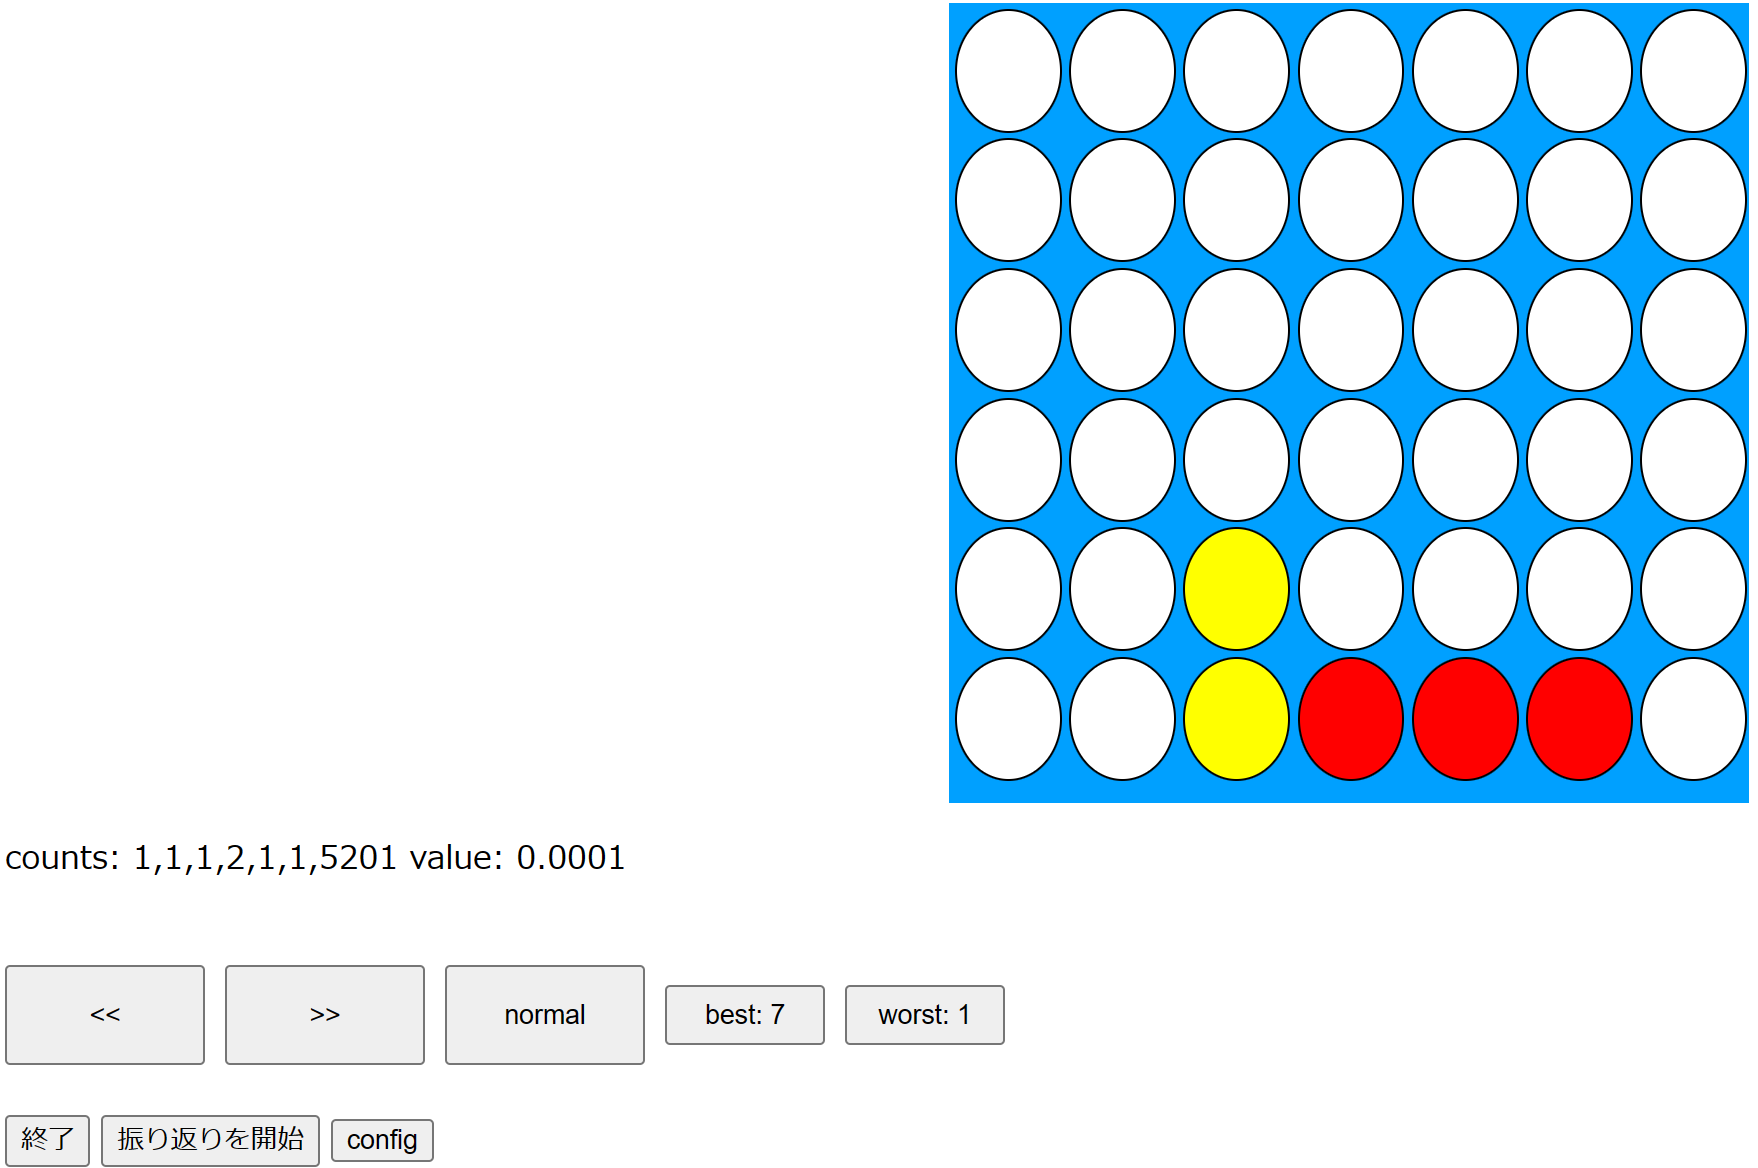
\includegraphics[width=\linewidth]{./figure/best-worst.png}
	\caption{進行図表示ボタン(2日目)}
	\label{fig:best-worst}
\end{figure}
\section{第2段階}
第2段階は提案手法を用いて振り返りを行ったグループ(A)の被験者と比較手法を用いて振り返りを行ったグループ(B)の被験者の対戦である.
1回の実験の中で2人の被験者が手番を入れ変え2回の対戦を行った.
制限時間は1ゲーム5分であり,制限時間内に終わらなかったゲームはAIによって判定した.具体的には制限時間が切れた際の盤面$s$のAIによる局面評価$V(s)$の絶対値が0.5以上である場合に
はその符号が示すプレイヤーの勝利とし,$V(s)$の絶対値が0.5未満である場合は引き分けとする.
判定用に使用したAIモデルのパラメータは\ref{table:param-judge}に示す.
\begin{table}[H]
	\caption{AIモデルのパラメータ(システム実験・第2段階)}
    \label{table:param-judge}
	\centering
	\scalebox{0.98}[0.98]{
		\begin{tabular}{c|c}
			パラメータ名 & 値 \\ \hline
			time    & 0\\ 
			$C_{puct}$    & 1 \\
            エポック数 & 200 \\
		\end{tabular}
	}
	
\end{table}


\section{質問項目の詳細}
質問項目は「タスクの熟達度に関連する質問」((a))と「タスクの楽しさ・面白さに関連する質問」((b))の2つに分けられる.
具体的な質問項目は\ref{table:query}に記載した.また,2日目は「タスクの楽しさ・面白さに関連する質問」に
「1回目と比べて成長したと感じますか」を追加した.
\begin{table}[H]
    \caption{質問項目:システム実験}
    \label{table:query}
    \centering
	\scriptsize
    \begin{tabular}{c||l}
        \multicolumn{1}{c|}{質問の種類} & \multicolumn{1}{c}{質問の内容} \\ \hline \hline
        \multicolumn{1}{c||}{}&対局によって成長したと感じましたか \\
        タスクの熟達度に関連する質問 & 振り返りによって成長したと感じましたか \\
		\multicolumn{1}{c||}{}&振り返りによってAIの意図を掴むことができたと感じますか \\
		\multicolumn{1}{c||}{} & (2日目のみ)1回目と比べて成長したと感じますか\\\hline
        \multicolumn{1}{c||}{} & 今後もconnect4をプレイするときにこのシステムを使いたいと思いましたか \\
        タスクの楽しさ・面白さに関連する質問 & システムにより振り返りが楽しくなったと感じますか\\
    \end{tabular}
    
\end{table}
\section{結果データ}
第4章では先読みの手数ごとに結果データを集計した.ここでは他の観点から集計されたデータを示す.
表\ref{table:system-all}に先読みの手数を分けずに合計した結果を示す.
\begin{table}[H]
    \caption{結果:総合}
    \label{table:system-all}
    \scriptsize
    \centering
    \resizebox{\linewidth}{!}{
        \begin{tabular}{c|l||c|c}
            \multicolumn{2}{c}{質問} & \multicolumn{2}{c}{主観評価} \\ \hline \hline
            質問の種類 & 質問の内容 & A & B \\ \hline 
            (a) & 振り返りによって成長したと感じましたか & 3.55 & \bf{3.86} \\
            & 振り返りによってAIの意図を掴むことができたと感じますか & 2.73 & \bf{3.32} \\
            & (2回目のみ) 1回目に比べて成長したと感じますか & 3.36 & \bf{4.00} \\ \hline
            (b) & 今後も connect4 をプレイするときにこのシステムを使いたいと思いましたか & 4.05 & \bf{4.27} \\
            & システムにより振り返りが楽しくなったと感じますか & 3.86 & \bf{4.33} \\
        \end{tabular}
    }
    
\end{table}

また,AIの強さごとに集計した結果を表\ref{table:system-strong},表\ref{table:system-weak}に示す.
表\ref{table:system-strong}に強いAIを用いて訓練した被験者のデータ,表\ref{table:system-weak}に
弱いAIを用いて訓練した被験者のデータを示す.
\begin{table}[H]
    \caption{結果:AIの強さ(強い)}
    \label{table:system-strong}
    \scriptsize
    \centering
    \resizebox{\linewidth}{!}{
        \begin{tabular}{c|l||c|c}
            \multicolumn{2}{c}{質問} & \multicolumn{2}{c}{主観評価} \\ \hline \hline
            質問の種類 & 質問の内容 & A & B \\ \hline 
            (a) & 振り返りによって成長したと感じましたか & 3.67 & \bf{3.82} \\
            & 振り返りによってAIの意図を掴むことができたと感じますか & 2.58 & \bf{3.55} \\
            & (2回目のみ) 1回目に比べて成長したと感じますか & 3.00 & \bf{4.00} \\ \hline
            (b) & 今後も connect4 をプレイするときにこのシステムを使いたいと思いましたか & 4.08 & \bf{4.64} \\
            & システムにより振り返りが楽しくなったと感じますか & 3.75 & \bf{4.50} \\
        \end{tabular}
    }
    
\end{table}

\begin{table}[H]
    \caption{結果:AIの強さ(弱い)}
    \label{table:system-weak}
    \scriptsize
    \centering
    \resizebox{\linewidth}{!}{
        \begin{tabular}{c|l||c|c}
            \multicolumn{2}{c}{質問} & \multicolumn{2}{c}{主観評価} \\ \hline \hline
            質問の種類 & 質問の内容 & A & B \\ \hline 
            (a) & 振り返りによって成長したと感じましたか & 3.8 & \bf{3.33} \\
            & 振り返りによってAIの意図を掴むことができたと感じますか & 3.00 & 3.00 \\
            & (2回目のみ) 1回目に比べて成長したと感じますか & 3.80 & \bf{4.00} \\ \hline
            (b) & 今後も connect4 をプレイするときにこのシステムを使いたいと思いましたか & \bf{4.00} & 3.80 \\
            & システムにより振り返りが楽しくなったと感じますか & 4 & \bf{4.1} \\
        \end{tabular}
    }
    
\end{table}
また,1日目のデータを表\ref{table:system-day1},2日目のデータを表\ref{table:system-day2}に記載する.
\begin{table}[H]
    \caption{結果:1日目}
    \scriptsize
    \centering
    \resizebox{\linewidth}{!}{
        \begin{tabular}{c|l||c|c}
            \multicolumn{2}{c}{質問} & \multicolumn{2}{c}{主観評価} \\ \hline \hline
            質問の種類 & 質問の内容 & A & B \\ \hline 
            (a) & 振り返りによって成長したと感じましたか & 3.56 & \bf{3.78} \\
            & 振り返りによってAIの意図を掴むことができたと感じますか & \bf{3.05} & 2.94 \\ \hline
            (b) & 今後も connect4 をプレイするときにこのシステムを使いたいと思いましたか & 4.06 & \bf{4.28} \\
            & システムにより振り返りが楽しくなったと感じますか & 4.06 & \bf{4.28} \\
        \end{tabular}
    }
    \label{table:system-day1}
\end{table}

\begin{table}[H]
    \caption{結果:2日目}
    \label{table:system-day2}
    \scriptsize
    \centering
    \resizebox{\linewidth}{!}{
        \begin{tabular}{c|l||c|c}
            \multicolumn{2}{c}{質問} & \multicolumn{2}{c}{主観評価} \\ \hline \hline
            質問の種類 & 質問の内容 & A & B \\ \hline 
            (a) & 振り返りによって成長したと感じましたか & 3.55 & \bf{3.91} \\
            & 振り返りによってAIの意図を掴むことができたと感じますか & 2.45 & \bf{3.64} \\ 
			& (2回目のみ) 1回目に比べて成長したと感じますか & 3.36 & \bf{4.00} \\ \hline
            (b) & 今後も connect4 をプレイするときにこのシステムを使いたいと思いましたか & 4.00 & 4.18 \\
            & システムにより振り返りが楽しくなったと感じますか & 3.91 & \bf{4.40} \\
        \end{tabular}
    }
    
\end{table}


